\section{T11 Retrospective}

We still had issues with reviewing and getting the text in the report. However, we did not experience the same problems with the inability to tell progress as in sprint 2.

Since the last sprint, the \gls{PR} process has been smoother, which is likely a result of loosening the rules a little, and the team members getting more used to the merging process. In sprint 3, we were better at answering each other when we worked from home, but not enough.

During sprint 3, we tried to invert the primary work area of each group member. We had some problems with this inversion due to three factors. Firstly, the user stories we got were either blocked for an extended period or were canceled. Secondly, we found it difficult to replace the canceled user stories. Finally, the members that usually work on the code got asked to help other groups a lot of the time, which resulted in the members having approximately the same roles in this sprint as in the last, which also relates to the final point of the previous retrospective because we were unsuccessful in redirecting other groups to \gls{POT}.

\subsection{Issues From This Sprint}

We did not meet at the university as much during sprint 3 because of the Easter holiday, and therefore we did not have a lot to talk about in this retrospective, but there was one issue.

\begin{figure}[ht]
    \centering
    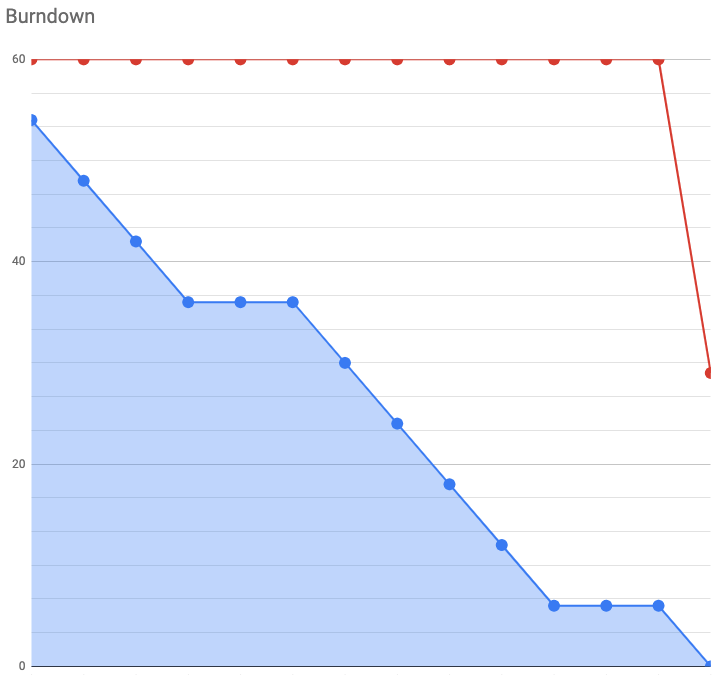
\includegraphics[width=0.5\textwidth]{figures/burndown.png}
    \caption{The burndown chart for sprint 3, blue meaning expected, red meaning actual burnrate.}
    \label{fig:burndown-chart}
\end{figure}

We made a sprint backlog at the beginning of the sprint where we put tasks we wanted to do during the sprint. We made a burndown chart for the backlog, which we can see in \autoref{fig:burndown-chart}, which showed two things: Firstly, we only finished about half the tasks planned, which indicates unrealistic planning, which we want to avoid in sprint 4. Secondly, we finished almost all tasks within the last days of the sprint, rather than evenly throughout the sprint.

Resolving the issue of finishing tasks at the end of the sprint, we appointed a member of our \gls{devTeam} the authority of assigning reviews to members, we called this role, the \textit{review master}.

\subsection{Things That Went Well}

We are good at communicating issues, and there is a high degree of respect in the group. Although we have small problems with our planning, we work hard. Since the last sprint, we have only gotten better at working together.
